
\documentclass[journal,11pt,onecolumn,draftclsnofoot]{ieeeconf}  % Comment this line out if you need a4paper

\usepackage{listings}
\usepackage{hyperref}
\usepackage{url}
\usepackage[pdftex]{graphicx}
\usepackage{amsfonts}
\usepackage{subfigure} 
\usepackage{algorithm}
%\usepackage{algorithmic}
\usepackage{amsmath}
\usepackage{bm}
\usepackage{algcompatible}
\usepackage{framed}
\usepackage{balance}

\usepackage{graphics} % for pdf, bitmapped graphics files
\usepackage{caption}
\usepackage{epsfig}
\usepackage{wrapfig}
\usepackage{breqn}
\newcommand{\myalpha}{\alpha_\rho}
\DeclareMathOperator*{\argmax}{arg\,max}

\pdfminorversion=4

\IEEEoverridecommandlockouts                              % This command is only needed if 
                                                          % you want to use the \thanks command
\overrideIEEEmargins                                      % Needed to meet printer requirements.

\author{Wenbo Xu, Wenwen Zhang, Yichi Zhang}

\title{
	EE 382C: Multicore Computing \protect\\
	\Large \bf Parallel GPU based Algorithms for Image Processing
}

\begin{document}
\maketitle
\thispagestyle{empty}
\pagestyle{empty}


\section{Abstract}
  

\section{Introduction}
Recently, the requirement for GPU (graphics processing unit) performance is increasing rapidly as well as the computation speed. As comparison, GPU computation speed can be several times faster than traditional CPU. Moreover, as the programmability and parallel processing emerge\cite{1}, GPU begins being used in some non-graphics applications, which is general-purpose computing on the GPU (GPGPU). To be more user-friendly, CUDA brings the C-like development 
environment and some CUDA extended libraries to programmers, which is based on industry-standard C/C++ and has straightforward APIs to manage devices, memory etc.

As an general use of GPU, Image processing algorithms are always computationally expensive, however, parallelize image processing algorithms can enhance the speed to a great extent, especially for large-scale images.

In this paper, we?

\section{Gaussian blur}
\subsection{Definition and Usage}
In image processing, a Gaussian blur (also known as Gaussian smoothing) is the result of blurring an image by a Gaussian function. It is a widely used effect in graphics software, typically to reduce image noise and reduce detail. 

Mathematically, the Gaussian blur is a type of image-blurring filter that uses a Gaussian function for calculating the transformation to apply to each pixel in the image.  For our implementation, we use a two-dimensions gaussian blur to filter each image pixel. The related two-dimensions gaussian function is the product of two such one-dimension function above, on in each dimention. 
  \[G(x) = \frac{1}{ \sqrt{2 \pi   \sigma ^{2} } } e^{ -\frac{ x^{2} +  y^{2}}{2  \sigma ^{2} }}\]
 Variable $x$ is the distance from the origin in the horizontal axis, $y$ is the distance from the origin in the vertical axis, and $\sigma$ is the standard deviation of the Gaussian distribution. A convolution matrix is built with values generated by this distribution.  
 To have a better view of the powerfulness of parallel computing, we did a comparison experiment, which is comprised with two implementations of Gaussian blur. One is sequential implementation and the other is parallel implementation. 

\subsection{Sequential  Implementation}
There are four steps of the sequential implementation. The first step is preprocess, which is responsible for reading image file and store it as Image class. The second step is to generate a gaussian filter, a matrix, based on parameters, like the standard deviation,  passed from users. The next step is to traverse each pixel in the image object and compute the values of a given pixel in the output image by multiplying each kernel value by the corresponding input image pixel values. The final step is to generate an image file from those new pixel values.

\subsection{Parallel  Implementation}
In this chapter, we implemented a normal parallel version gaussian blurring based on CUDA. In the following chapter, we optimized this implementation in several ways.  Firstly, we read the image file and generate filter matrix. Then we need to copy the image into device memory. Each pixel is combined with three channels, $r$, $g$ and $b$.  They should be separated and be gaussian blurred separately. Then we start the kernel three times and do gaussian blurring to each channel per time.  At last, we copy three blurred channels from device to host and save them into an image file.This process is described with the Fig.1.

\begin{figure}[h]
	\centering\includegraphics[width=85mm,height=80mm]{ImageProcessingCuda.png}
	\caption{Diagram for Parallel Image Processing}
	\label{parallel}
\end{figure}


\section{Optimization}

\subsection{Shared memory v.s. Global Memory}
In the previous version implementation of Gaussian blur, we store three channels in global memory, and access same global memory several times when we read neighbour channels. Since reading shared memory is much faster (shared memory ~$1.7TB/s$, while global memory ~ $150GB/s$), instead of pulling from global memory every time, we put channel values in the shared memory for other threads within the same block to see and reuse. 

In order to compute blurred channel values at the boundary of one block, we need to load channel values from neighboring blocks, so shared memory size should be a little larger than a block size and threads at the boundary area are responsible for loading channel values from neighboring blocks. This is displayed at Fig.2. Threads in blue area of dotted square are responsible for loading channel values from corresponding white area.

\begin{figure}[h]
	\centering\includegraphics[width=120mm,height=85mm]{SharedMemory.png}
	\caption{Loading neighbour channel values for shared variable}
	\label{parallel}
\end{figure}

\subsection{Pageable v.s. Pinned Memory}
Host data allocations are pageable by default, However, GPU cannot access data directly from pageable memory, but from pinned memory. As shown in Figure \cite{Mark}, whenever a data transfer is invoked on pageable memory, the CUDA driver has to allocate a temporary pinned memory array to copy host data and then transfer it to the device. \par
\begin{figure}[h]
	\centering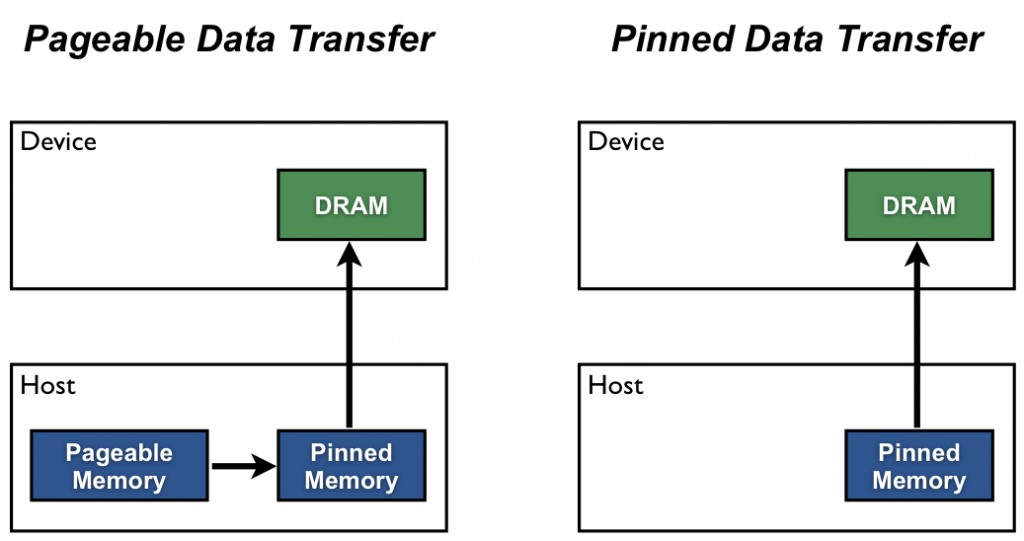
\includegraphics[width=120mm]{pinned.jpg}
	\caption{CUDA data transfer.\cite{Mark}}
	\label{CUDA data transfer.}
\end{figure}
We can use \textit{cudaMallocHost()} and \textit{cudaFreeHost()} instead of \textit{malloc()} and \textit{free()}, to remove the overhead described above. However, \textit{cudaMallocHost()} and \textit{cudaFreeHost()} are more expensive with additional overheads. According to Boyer\cite{Trade_off}, pinned memory is faster when the size of data to be transfered is larger than 16MB. \par

\subsection{Streams}
A stream is defined as a sequence of operations in that execute in issue-order on the GPU. A typical CUDA task consists of three operations, memcpy HToD, kernel, and memcpyDToH. Kernel operations in different streams may run concurrently as long as the hardware resources were available. For memory copies, one transfer per direction is allowed at any time. And memory copies in different streams are in different direction may run concurrently when hardware supports two copy engine.   \par

Figure \ref{concurrent} illustrates the execution time line for three different scenarios. In this project, the pipelined fashion was implemented. In order to pipeline the memory copies, asynchronous memory copiy functions, \textit{cudaMemcpyAsync()}, are used instead of synchronous functions.\cite{Stream} \par

\section{Results}
Both CPU and GPU implementations was running on the TACC Stampede Supercomputer. The CPU is Intel® Xeon® E5-2680 2.7GHz Processors. And the GPU is NVIDIA K20 with 5120 MB GDDR5 memory and 2 copy engines. \par
The command line tool, nvprof, and the Nvidia Visual Profiler are used to profile the performance of our implementation. And the results are shown in Figure \ref{performances}.

\begin{figure}[h]
	\centering
	\fbox{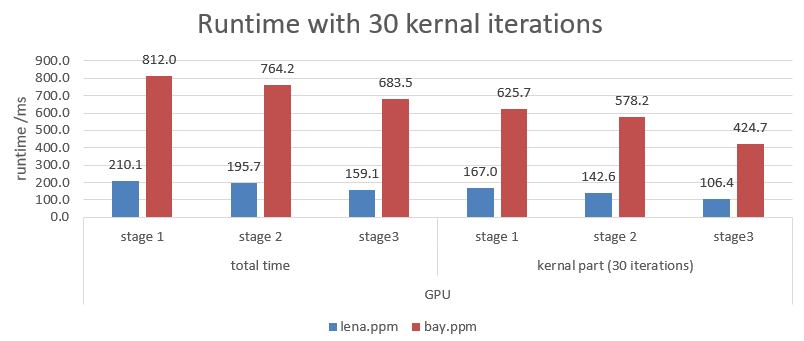
\includegraphics[width=120mm]{chart.PNG}}
	\caption{Performance Improvement in GPU.}
	\label{performances}
\end{figure}

\section{Conclusion} 
In our project, we implemented Gaussian Filter to two images, lena.ppm$(512*512)$ and bay.ppm$(1024*1024)$ in both CPU sequential logic and GPU parallel logic. After making it work correctly, we implemented three improvements:  \\
1.����� We changed allocation method from allocating pageable memory to pinned memory \\
2.����� We modified sequential kernel execution into pipelined execution \\
3.����� We replaced global kernel method with shared memory method \\

According to the theory of Gaussian Filter, we started with implementing sequential algorithm in pure CPU environment. The original image and executed result image for lena.ppm(small-scale) are show in appendix. We executed Gaussian blurring 30 times in order to better compute speed up later and the execution time is 16.6s.

Then, we changed the memory allocation method by using cudaMallocHost instead of malloc, after that, the modified execution time is 167.0ms. As can see the performance is much enhanced compared to the pure sequential logic.
Next, since we found that the kernel took much percentage of the whole execution time, we pipelined the kernel method execution to further improve the performance. After that, the modified execution time is 142.6. From the View Profiler, we noticed that it did pipeline a little bit but not as expected as we wanted. After researching, the reason is that for K20[?] , there is a limitation number of blocks(180) run on the same and to execute the kernel method, we need 256 blocks which means we need to wait for an amount of blocks to finish their current task, only after that can we reuse the source and execute the next kernel method. The profiler results for non-pipeline verses pipeline is show in Figure \ref{viewer}.

\begin{figure}[!tbp]
	\centering
	\begin{minipage}[b]{1\textwidth}
		\fbox{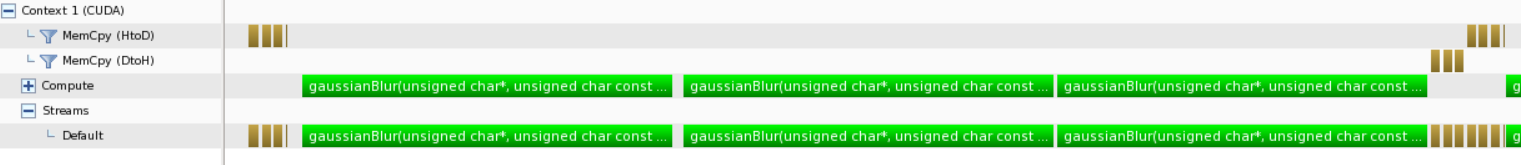
\includegraphics[width=160mm, height=40mm]{stage1.PNG}}
	\end{minipage}
	\begin{minipage}[b]{1\textwidth}
		\boxed{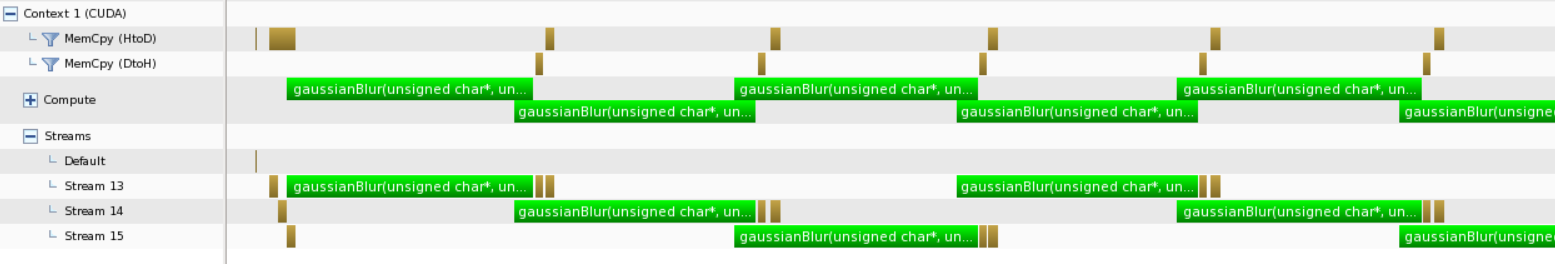
\includegraphics[width=160mm, height=60mm]{stage3.PNG}}
	\end{minipage}
	
	\caption{Time profiler viewer without using streams(top) verses using streams(bottom)}
	\label{viewer}
\end{figure}
Finally, we used shared memory to avoid wasting time to read from global memory each time, and thus further improved the performance. Our final execution time for lena.ppm is 106.4ms, which speeded up 156x(16.6s/106.4ms) from the very beginning.

\clearpage
\appendix
\section{Appendix}
\begin{figure}[h]
	\centering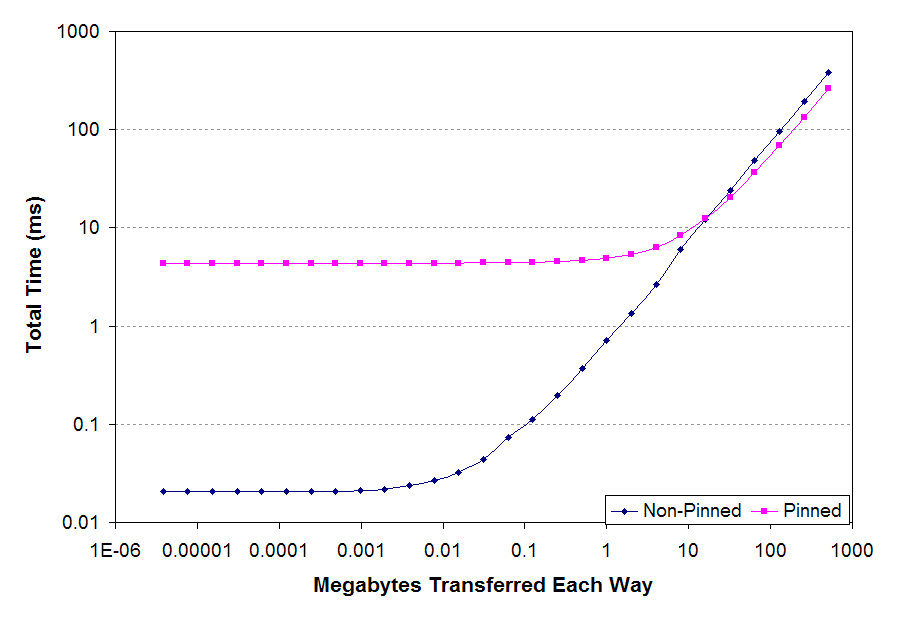
\includegraphics[width=120mm]{pinned_trade_off.png}
	\caption{Time required to allocate, transfer to the GPU, transfer back to the CPU, and deallocate pinned and non-pinned memory.\cite{Trade_off}}
	\label{Time required to allocate, transfer to the GPU, transfer back to the CPU, and deallocate pinned and non-pinned memory.}
\end{figure}
\begin{figure}[h]
	\centering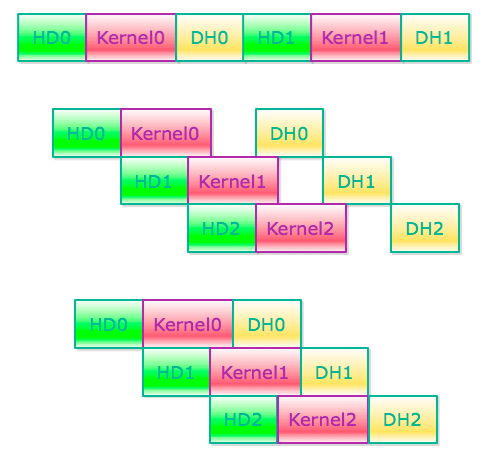
\includegraphics[width=120mm]{concurrent.png}
	\caption{Top: all operation in default stream. Mid: concurrent streams with one copy engine. Bottom: concurrent streams with two copy engine.}
	\label{concurrent}
\end{figure}

\clearpage
\bibliographystyle{abbrv}
\begin{thebibliography}{9}
\bibitem{1}
WU En Hua , ?State of the Art and Future Challenge on General 
Purpose Computation by Graphics Processing Unit?, Journal of 
Software, vol. 15, no. 10, 2004,pp.1493~1504.

\bibitem{Mark} 
Harries, M. (2012, December). How to Optimize Data Transfers in CUDA C/C++. Retrieved from https://devblogs.nvidia.com/parallelforall/how-optimize-data-transfers-cuda-cc/
	
\bibitem{Trade_off} 
Boyer, M. Choosing Between Pinned and Non-Pinned Memory. Retrieved from https://www.cs.virginia.edu/~mwb7w/cuda_support/pinned_tradeoff.html
	
\bibitem{Stream} 
Harries, M. (2012, December). How to Overlap Data Transfers in CUDA C/C++. Retrieved from https://devblogs.nvidia.com/parallelforall/how-overlap-data-transfers-cuda-cc/
	

\end{thebibliography}

\end{document}